
\section{Data}

Historical weather data is available from the Daily Global Historical Climatology Network \citep{Menne_2012}. This includes daily minimum and maximum temperature and daily precipitation. They provide data for about 1200 measurement stations across the United States. Based on the stations' coordinates they can be matched to the county they are in. Thus, temperature data can easily be aggregated to the county level. For counties with more than one measurement station, I take the mean among those.

Similar to \citet{Habeeb_2015} I define an extreme heat event as any day on which the temperature exceeds the 85th percentile of July and August temperatures. The quantile can be varied as a robustness check.

The National Highway Traffic Safety Administration provides data on fatal car accidents in their Fatality Analysis Reporting System (FARS). This includes every fatal accident between 1975 and 2020, including date and county information.


\begin{figure}[h]
	\centering
	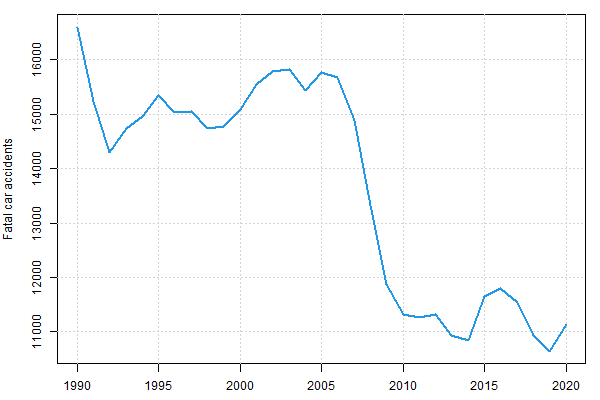
\includegraphics[scale = 0.5]{"../Code & Data/FatalAccidentsYearly.png"}
	\caption{Fatal car accidents by year}
\end{figure} 

